%% bare_jrnl.tex
%% V1.4b
%% 2015/08/26
%% by Michael Shell
%% see http://www.michaelshell.org/
%% for current contact information.
%%
%% This is a skeleton file demonstrating the use of IEEEtran.cls
%% (requires IEEEtran.cls version 1.8b or later) with an IEEE
%% journal paper.
%%

\documentclass[journal,onecolumn]{IEEEtran}
%
% If IEEEtran.cls has not been installed into the LaTeX system files,
% manually specify the path to it like:
% \documentclass[journal]{../sty/IEEEtran}

\usepackage[pdftex]{graphicx}
\usepackage{amsmath}
\usepackage{amssymb}
\usepackage{algpseudocode}
\usepackage{algorithm}
\usepackage{xpatch}
\usepackage{cite}
\usepackage{tikz}
\usetikzlibrary{shapes, arrows}

%\usepackage{array}
%\usepackage[caption=false,font=normalsize,labelfont=sf,textfont=sf]{subfig}
%\usepackage{url}

\hyphenation{op-tical net-works semi-conduc-tor}

%% For algorithms...
\algrenewcommand\alglinenumber[1]{{\sffamily\footnotesize#1:}}
\makeatletter
\xpatchcmd{\algorithmic}{\itemsep\z@}{\itemsep=5pt}{}{}
\makeatother
\renewcommand{\algorithmicrequire}{\textbf{Input:}}
\renewcommand{\algorithmicensure}{\textbf{Output:}}
\renewcommand{\algorithmicforall}{\textbf{For Each}}

% Define block styles for tikz...
\tikzstyle{decision} = [diamond, draw, fill=blue!20, text width=4.5em, 
    text centered, node distance=3cm, inner sep=0pt]
\tikzstyle{block} = [rectangle, draw, fill=blue!20, text width=3cm, 
    text centered, rounded corners, minimum height=4em]
\tikzstyle{info} = [rectangle, scale=0.6, text width=5cm, minimum height=4em, node distance=5.5cm]
\tikzstyle{line} = [draw, -latex']
\tikzstyle{cloud} = [draw, ellipse,fill=red!20, node distance=3cm,
    minimum height=2em]
\tikzstyle{io} = [trapezium, trapezium left angle=70, trapezium right angle=110, 
    minimum height=1cm, text centered, draw=black, fill=blue!30]

\begin{document}
% \title{_}
% \author{_}
% 
% \maketitle

\section{Methods}
%\IEEEPARstart{T}{his} 
This section explains two alternative methodologies to find moving flock patterns in large spatio-temporal datasets using modern distributed frameworks to divide and parallelize the work load.

\subsection{The BFE algorithm}
The first alternative follows closely the steps explained at \cite{vieira_2009}.  In this work, the authors proposed the Basic Flock Evaluation (BFE) algorithm to find flock pattern on trajectories databases.  The details of the algorithm can be accessed at the source but figure \ref{fig:flowchart1} explains schematically the work flow where we can identify 4 general steps:

\begin{enumerate}
    \item Pair finding:  Using the $\varepsilon$ parameter, the algorithm query the set of points to get the set of pairs which laid at a maximum distance of $\varepsilon$ units.  Usually, it is a distance self-join operation over the set of points using $\varepsilon$ as the distance parameter.  The query also pays attention to do not return pair duplicates.  Pair between point $p_1$ and $p_2$ is the same that pair between $p_2$ and $p_1$ and just one of them should be reported (the id of each point is used to filter duplicates).
    \item Center computation:  From the set of pairs of points available, each tuple is the input of a simple computation to locate the centers of the two circles of radius $\frac{\varepsilon}{2}$ which circumference laid on the input points.  The pseudocode of the procedure can be seen in appendix \ref{app:centers}.
    \item Disk finding: Once the centers have been identified, a query to collect the points around those centers is needed in order to group the set of points which laid $\varepsilon$ distance unit each other.  This is done by running a distance join query between the set of points and the set of centers using $\frac{\varepsilon}{2}$ as the distance parameter. Therefore, a disk will be defined by its center and the IDs of the points around it. At this stage, a filter is applied to remove those disks which collect less than $\mu$ elements around it.
    \item Disk pruning: It is possible than a disk collects the same set of points, or a subset, of the set of points of another disk.  In such cases, the algorithm should report just that one which contains the others.  An explanation of the procedure can be seen in appendix \ref{app:disks}.
\end{enumerate}

\begin{figure}[b]
    \centering
    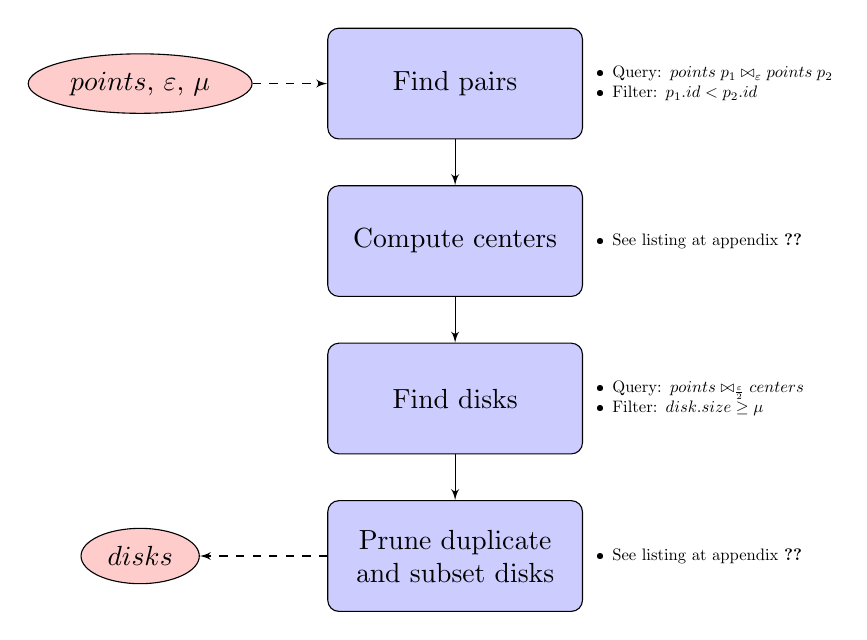
\begin{tikzpicture}[node distance = 2cm, auto]
        % Place nodes
        \node [block] (pairs) {Find pairs};
        \node [cloud, node distance=4cm, left of=pairs] (input) {$points$, $\varepsilon$, $\mu$};
        \node [block, below of=pairs] (centers) {Compute centers};
        \node [block, below of=centers] (disks) {Find disks};
        \node [block, below of=disks] (maximals) {Prune duplicate and subset disks};
        \node [cloud, node distance=4cm, left of=maximals] (output) {$disks$};
        % Info nodes
         \node [info, right of=pairs] (pairs_info) {
            \textbullet \hspace{0.1em} Query: $points\;p_1 \bowtie_{\varepsilon} points\;p_2$ \\
            \textbullet \hspace{0.1em} Filter: $p_1.id < p_2.id$ 
         };
        \node [info, right of=centers] (centers_info) { 
            \textbullet \hspace{0.1em} See listing at appendix \ref{app:centers}
        };
        \node [info, right of=disks] (disks_info) {
            \textbullet \hspace{0.1em} Query: $points \bowtie_{\frac{\varepsilon}{2}} centers$ \\
            \textbullet \hspace{0.1em} Filter: $disk.size \geq \mu $ 
         };
        \node [info, right of=maximals] (maximals_info) { 
            \textbullet \hspace{0.1em} See listing at appendix \ref{app:disks} 
        };
        % Draw edges
        \path [line,dashed] (input) -- (pairs);
        \path [line] (pairs) -- (centers);
        \path [line] (centers) -- (disks);
        \path [line] (disks) -- (maximals);
        \path [line,dashed] (maximals) -- (output);
    \end{tikzpicture}
    
    \caption{General steps in BFE algorithm.}\label{fig:flowchart1}
\end{figure}

It is important to note that BFE also proposes a grid index structure to speed up spatial operations.  The algorithm divides the space area in a grid of $\varepsilon$ side (see figure \ref{fig:grid}).  In this way, BFE just processes each grid and its 8 neighborhood grids.  It does not need to query grids outside of its neighborhood given that points in other grids are far away to affect the results.

\begin{figure}
    \centering
    \includegraphics[clip,trim=13cm 21.75cm 4.1cm 1.85cm]{figures/grid}
    \caption{The grid-based index structure proposed at \cite{vieira_2009}.}\label{fig:grid}
\end{figure}

\newpage

\begin{figure}[h!]
    \centering
    \includegraphics[width=\textwidth]{figures/MF_stages/P123}
    \caption{About partitioning and replication.}\label{fig:partrep}
\end{figure}

\begin{figure}[h!]
    \centering
    \includegraphics[width=\textwidth]{figures/MF_stages/flow}
    \caption{Local work.}\label{fig:example}
\end{figure}

\newpage 

\appendices
\section{Center computation.}\label{app:centers}

\alglanguage{pseudocode}
\begin{algorithm}
    \caption{Find the centers of given radius which circumference laid on the two input points.}
    \begin{algorithmic}[1]
        \Require Radius $\frac{\varepsilon}{2}$ and points $p_1$ and $p_2$.
        \Ensure Centers $c_1$ and $c_2$.
        
        \Function{FindCenters}{$p_1$, $p_2$, $\frac{\varepsilon}{2}$}
        \State $r^2 \gets (\frac{\varepsilon}{2})^2$
        \State $X \gets p_1.x - p_2.x$
        \State $Y \gets p_1.y - p_2.y$
        \State $d^2 \gets X^2 + Y^2$
        \State $R \gets \sqrt{\lvert 4 \times \frac{r^2}{d^2} - 1 \rvert}$
        \State $c_1.x \gets X + \frac{Y \times R}{2} + p_2.x$
        \State $c_1.y \gets Y - \frac{X \times R}{2} + p_2.y$
        \State $c_2.x \gets X - \frac{Y \times R}{2} + p_2.x$
        \State $c_2.y \gets Y + \frac{X \times R}{2} + p_2.y$
        
        \State \Return $c_1$ and $c_2$
        \EndFunction
    \end{algorithmic}
\end{algorithm}

\newpage

\section{Disk prunning.}\label{app:disks}

\begin{algorithm}
    \caption{Prune disks which are duplicate or subset of others.}
    \begin{algorithmic}[1]
        \Require Set of disks $D$.
        \Ensure Set of disks $D^{\prime}$ without duplicate or subsets.
        
        \Function{pruneDisks}{$D$}
        \State $E \gets \varnothing$
        \ForAll{disk $d_i$ in $D$}
            \State $N \gets d_i \cap D$
            \ForAll{disk $n_j$ in $N$}
                \If{$d_i$ contains all the elements of $n_j$}
                        \State $E \gets E \cup {n_j}$
                \EndIf
            \EndFor
        \EndFor        
        \State $D^{\prime} \gets D \setminus E$
        \State \Return $D^{\prime}$
        \EndFunction
    \end{algorithmic}
\end{algorithm}

\bibliographystyle{IEEEtran}
\bibliography{../pflocks.bib}

\end{document}
